\section{Results}
\label{section:results}

We have implemented the algorithm in Section \ref{section:algorithm}
in a tool called \texttt{CRTSolver} which is available at
\url{https://github.com/maheenmatin/CRTSolver} under LICENSE-GOES-HERE.
%
It uses two instances of cvc5, one to solve the modulo sub-problems
and a second to check the candidate results.  The following options
are available: Integer Mode and Bit-Vector Mode. 

Integer Mode attempts to
solve the modulo subproblem using the theory of Quantifier-Free Nonlinear
Integer Arithmetic, where the variables are of integer sort and integer
operations are used. 
Bit-Vector Mode uses the theory of Quantifier-Free
Bit-Vector Logic, where the variables are of bit-vector sort (with a fixed
bit-width calculated as a function of the current prime) and bit-vector
operations are used.
For the checking of candidate results, the theory of Quantifier-Free
Nonlinear Integer Arithmetic is used for both Integer Mode and Bit-Vector
Mode.

We have created a set of benchmarks that evaluate the performance of CRTSolver 
in both available modes on non-linear integer equations, in comparison with two
widely used and state-of-the-art SMT solvers, Z3 and cvc5.
The benchmarks are time and success rate, where time simply refers to the total runtime
for a given equation in milliseconds. We define a successful solving of a given
equation as termination with \texttt{SAT} or \texttt{UNSAT} - if a solver terminates
with \texttt{UNKNOWN} due to time constraints, memory constraints, or internal error,
then we define this as an unsuccessful solving.


In Table \ref{table:results} we give a comparison with \mbsays{Say
  which solver and cite the relevant paper -- see their websites for
  which one}.
\mbsays{Describe the experimental set up: what hardware/processor, what operating system, what solver versions,  what time and memory limits.}
\mbsays{ If a solver times out
put T/O in the time, if it is out of memory put M/O, if it returns
UNKNOWN then put U.  You need to say here in the paper this is what
they mean.}
These results are also shown in a cactus plot in Figure \ref{figure:cactus-plot}.


\begin{table*}
  \caption{Performance Comparison between CRTSolver, Z3 and cvc5.}
  \label{table:results}
  \begin{tabular}{ccccccccc}
    \toprule
    Equation & Variables & Degree & SAT & CRT-INT & CRT-BV & Z3 & cvc5 \\
    \midrule
    ? & ? & ? & ? & ? & ? & ? & ? \\
    ? & ? & ? & ? & ? & ? & ? & ? \\
  \bottomrule
\end{tabular}
\end{table*}
\mbsays{Fill in the table.  Either use a program to generate it or
  maybe \url{https://www.tablesgenerator.com/}.}

\begin{figure*}
    \vspace{4em}
    \centering
    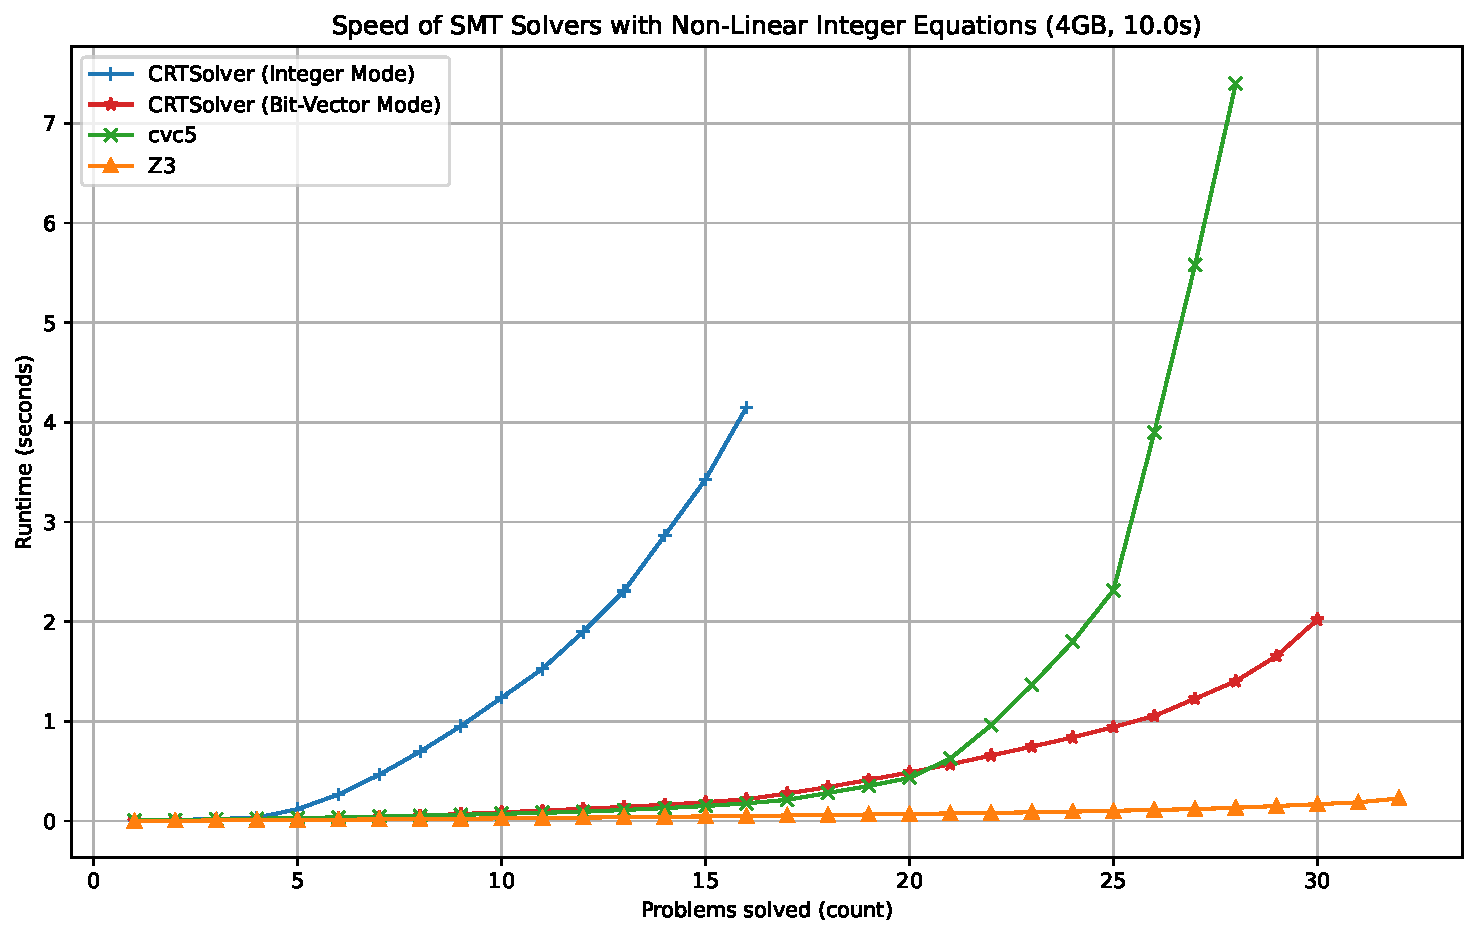
\includegraphics[width=1.0\linewidth]{cactus.pdf}
  \caption{A cactus plot of the results.}
  \label{figure:cactus-plot}
\end{figure*}
\mbsays{Create the cactus plot}

These result suggest that \mbsays{Write a paragraph or so about things
we can conclude.  For example, CRTSolver with bit-vectors is way
faster than with integer, they are both much faster than the other
solvers, there is a difference between SAT and UNSAT, etc. etc.}
